%************************************************
\chapter{Prove dinamico-meccaniche}\label{chp:DinamicoMeccaniche}
%************************************************
Consistono nell'imporre al materiale una storia di deformazione periodica nel tempo.
Ad esempio:
\begin{equation}
\epsilon(t) = \bar{\epsilon}\sin(\omega t)
\end{equation}
Assomiglia ad una prova di fatica per i metalli, ma ha tutt'altro significato.

Bastano alcuni minuti di sollecitazione a $\epsilon(t)$ per ottenere i dati caratteristici del materiale. Inoltre, in questo caso si controlla la deformazione e il materiale non si rompe.

I dati che si ottengono sono:
\begin{equation}
\begin{split}
\sigma(t) &= \epsilon(0)E(t) + \int_0^t{E(t-\tau)\dot{\epsilon}(s)\,ds}\\
E(t) &= E_{\infty} + \Delta E(t)
\end{split}
\end{equation}
Se il materiale è fluido viscoelastico allora $E_{\infty} = 0$, altrimenti $E_{\infty} > 0$.
Mente $\Delta E(t) \underrightarrow{t \rightarrow \infty} 0$.
Allora:
\begin{equation}
\begin{split}
\sigma(t) &= \epsilon(0)(E_{\infty} + \Delta E(t)) + \int_0^t{(E_{\infty} + \Delta E(t-s)) \dot{\epsilon}(s)\,ds}\\
&= \epsilon(0)E_{\infty} + \epsilon(0)\Delta E(t) + \int_0^t{E_{\infty}\dot{\epsilon}(s)\,ds} +  \int_0^t{\Delta E(t-s) \dot{\epsilon}(s)\,ds}\\
&= \epsilon(0)E_{\infty} + \epsilon(0)\Delta E(t) + E_{\infty}(\epsilon(t) - \epsilon(0)) + \int_t^0{\Delta E(\tau) \dot{\epsilon}(t-\tau)\,-d\tau}\\
&= \epsilon(0)\Delta E(t) + E_{\infty}\epsilon(t) + \int_0^t{\Delta E(s) \dot{\epsilon}(t-s)\,ds}\\
\end{split}
\end{equation}
Imponendo che $\epsilon(t) = \bar{\epsilon}\sin(\omega t)$ allora:
\begin{equation}
\begin{split}
\sigma(t) &= E_{\infty} \bar{\epsilon}\sin(\omega t) + \int_0^t{\Delta E(s)\omega\bar{\epsilon}\cos(\omega(t-s))\,ds}\\
&= E_{\infty} \bar{\epsilon}\sin(\omega t) + \omega\bar{\epsilon}\int_0^t{\Delta E(s) \left[\cos(\omega t)\cos(\omega s) + \sin(\omega t)\sin(\omega s)\right]\,ds}\\
&= E_{\infty} \bar{\epsilon}\sin(\omega t) + \omega\bar{\epsilon}\int_0^t{\Delta E(s) \cos(\omega t)\cos(\omega s)\,ds} +\\
&\omega\bar{\epsilon}\int_0^t{\Delta E(s)\sin(\omega t)\sin(\omega s)\,ds}\\
&= E_{\infty} \bar{\epsilon}\sin(\omega t) + \omega\bar{\epsilon}\cos(\omega t)\int_0^t{\Delta E(s) \cos(\omega s)\,ds} +\\
&\omega\bar{\epsilon}\sin(\omega t)\int_0^t{\Delta E(s)\sin(\omega s)\,ds}\\
&= \bar{\epsilon}\left[E_{\infty} + \omega\int_0^t{\Delta E(s)\sin(\omega s)\,ds}\right]\sin(\omega t) +\\
&\bar{\epsilon}\left[\omega\int_0^t{\Delta E(s)\cos(\omega s)\,ds}\right]\cos(\omega t)
\end{split}
\end{equation}
Sarebbe la storia di deformazione è sinusoidale, non è detto che la storia di sforzo lo sia.
\begin{equation}
\begin{split}
\int_0^t{\Delta E(s)\sin(\omega s)\,ds} \quad \overrightarrow{t \rightarrow \infty} \quad \exists \int_0^t{\Delta E(s)\sin(\omega s)\,ds} < \infty\\
\int_0^t{\Delta E(s)\cos(\omega s)\,ds} \quad \overrightarrow{t \rightarrow \infty} \quad \exists \int_0^t{\Delta E(s)\cos(\omega s)\,ds} < \infty\\
\end{split}
\end{equation}
\begin{equation}
\begin{split}
\sigma(t) &= \bar{\epsilon}\underbrace{\left[E_{\infty} + \omega\int_0^t{\Delta E(s)\sin(\omega s)\,ds}\right]}_{E'(\omega)}\sin(\omega t) +\\
&+\bar{\epsilon}\underbrace{\left[\omega\int_0^t{\Delta E(s)\cos(\omega s)\,ds}\right]}_{E"(\omega)}\cos(\omega t)
\end{split}
\end{equation}
Da cui:
\begin{equation}
\begin{cases}
\sigma(t) &= \bar{\epsilon} E'(\omega)\sin(\omega t) + \bar{\epsilon} E"(\omega)\cos(\omega t)\\
E'(\omega) &:=\textup{ Modulo conservativo}\\
E"(\omega) &:=\textup{ Modulo dissipativo}
\end{cases}
\end{equation}
Si riesce a vedere quanto il materiale è in grado di mantenere energia rispetto a quanto ne dissipi.

\begin{description}
\item[Modulo conservativo] parte in fase con la sollecitazione, rappresenta la capacità del materiale di conservare energia.
\item[Modulo dissipativo] parte in contro fase con la sollecitazione, rappresenta la capacità del materiale a dissipare energia. 
\end{description}

\section{Come viene realizzata la prova?}
Se la forzate è definita come: $\epsilon(t) = \bar{\epsilon}\sin(\omega t)$ allora lo sforzo può essere visto come: $\sigma(t) = \bar{\sigma}\sin(\omega t + \delta)$. Da cui:
\begin{equation}
\begin{split}
\sigma(t) &= \bar{\sigma}\left(\sin(\omega t)\cos(\delta) + \cos(\omega t)\sin(\delta)\right) =\\
&= \underbrace{(\bar{\sigma}\cos(\delta))}_{\bar{\epsilon}E'}\sin(\omega t) + \underbrace{(\bar{\sigma}\sin(\delta))}_{\bar{\epsilon}E"}\cos(\omega t)\\
\begin{cases}
E' &=\frac{\bar{\sigma}}{\bar{\epsilon}}\cos(\delta)\\
E" &=\frac{\bar{\sigma}}{\bar{\epsilon}}\sin(\delta)
\end{cases}
\end{split}
\end{equation}

\begin{figure}
\centering
\subfloat[][\emph{Componente conservativa}\label{fig:ComponenteConservativa}]
{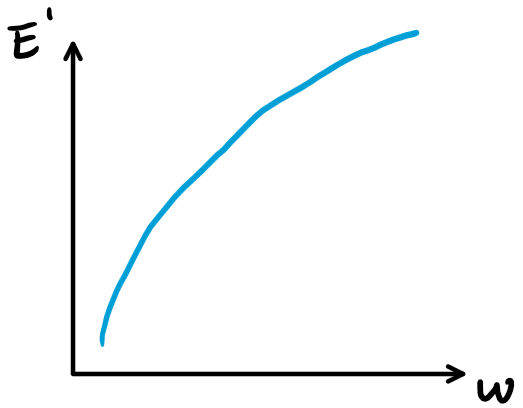
\includegraphics[width = 0.4\textwidth]{gfx/ComponenteConservativa}}\quad
\subfloat[][\emph{Componente dissipativa}\label{fig:ComponenteDissipativa}]
{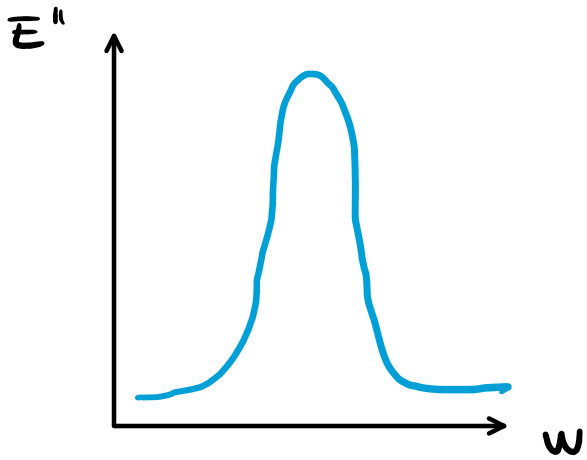
\includegraphics[width = 0.4\textwidth]{gfx/ComponenteDissipativa}}\\
\subfloat[][\emph{Combinazione sul materiale della deformazione e sforzo nella prova dinamica}\label{fig:Combinazione}]
{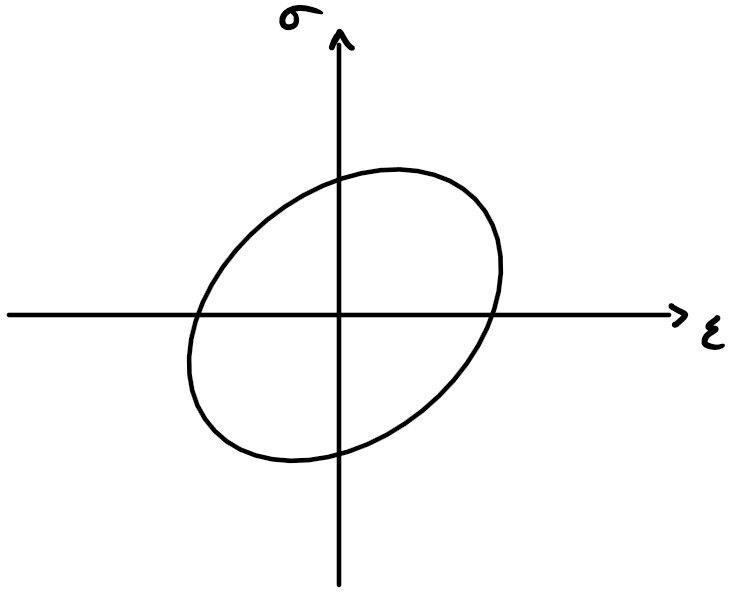
\includegraphics[width = 0.5\textwidth]{gfx/Combinazione}}
\caption{Componenti della prova dinamico-meccanica}
\label{fig:ComponentiProva}
\end{figure}

Dalla figura \ref{fig:ComponentiProva}, si osserva che le componenti hanno comportamento diverso tra loro.
\begin{description}
\item[Componente conservativa $E'$] ha un andamento crescente al crescere della frequenza della prova.
\item[Componente dissipativa $E"$] ha un andamento a campana, dunque per basse e alte frequenza tende a zero, ha un picco per frequenze intermedie.
\end{description}

Allora:
\begin{equation}
\begin{split}
\epsilon(t) &= \bar{\epsilon}\sin(\omega t) \doteq \omega \bar{\epsilon}\cos(\omega t)\\
\sigma(t) &= \bar{\sigma}\sin(\omega t + \delta)
\end{split}
\end{equation}
In termini energetici:
\begin{equation}
\begin{split}
W &= \int_{ciclo}\sigma\,d\epsilon\\
&= \int_t^{t+\frac{2\pi}{\omega}}{\sigma \frac{d\epsilon}{ds}\,ds}\\
W &= \int_t^{t+\frac{2\pi}{\omega}}{\bar{\sigma}\sin(\omega t + \delta) \cdot \omega \bar{\epsilon}\cos(\omega s)\,ds}\\
W &= \bar{\sigma} \bar{\epsilon}\omega\int_t^{t+\frac{2\pi}{\omega}}{\cos(\omega s)\left[\sin(\omega s)\cos(\delta) + \cos(\omega s)\sin(\delta)\right]\,ds}\\
&= \bar{\sigma}\bar{\epsilon}\omega\left[\cos(\delta)\int_t^{t+\frac{2\pi}{\omega}}{\cos(\omega s)\sin(\omega s)\,ds} + \sin(\delta)\int_t^{t+\frac{2\pi}{\omega}}{\cos^2(\omega s)\,ds}\right]\\
&=\bar{\sigma}\bar{\epsilon}\omega\sin(\delta)\frac{1}{2}\frac{2\pi}{\omega}\\
&= \bar{\sigma}\bar{\epsilon}\pi\sin(\delta) = \pi \bar{\epsilon}^2E"(\omega)
\end{split}
\end{equation}
Da cui si può definire il fattore di perdita come: $\frac{E"}{E'} = \tan(\delta)$.

\paragraph{Applicando al solido a tre parametri:}
\begin{equation}
E(t) = E_{\infty} + (E_0-E_{\infty})E^{-\frac{t}{\tau_r}}
\end{equation}
Da cui:
\begin{equation}
\begin{cases}
E'(\omega) &= E_{\infty} + \omega\int_0^{\infty}{(E_0-E_{\infty})e^{-\frac{t}{\tau_r}}\sin(\omega s)\,ds}\\
&= E_{\infty} + (E_0-E_{\infty})\frac{\omega^2\tau_r^2}{1+\omega^2\tau_r^2}\\
E"(\omega) &= \omega\int_0^{\infty}{(E_0-E_{\infty})e^{-\frac{t}{\tau_r}}\cos(\omega s)\,ds}\\
&= (E_0 - E_{\infty})\frac{\omega \tau_r}{1+\omega^2\tau_r^2}
\end{cases}
\end{equation}

\begin{figure}
\centering
\subfloat[][\emph{Componente conservativa per il modello a tre parametri}\label{fig:Conservativa3Param}]
{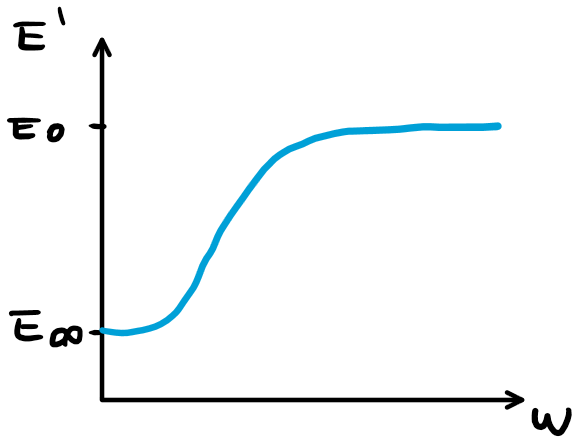
\includegraphics[width = 0.4\textwidth]{gfx/Conservativa3Param}}\quad
\subfloat[][\emph{Componente dissipativa per il modello a tre parametri}\label{fig:Dissipativa3Param}]
{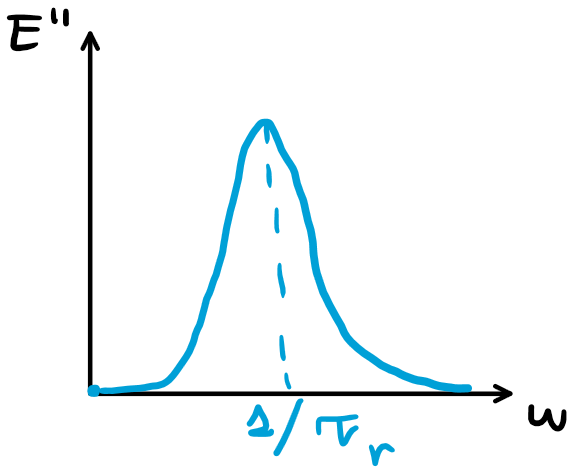
\includegraphics[width = 0.4\textwidth]{gfx/Dissipativa3Param}}
\caption{Risultati di un prova dinamica per un fluido a tre parametri}
\label{fig:3Param}
\end{figure}
Il tempo di rilassamento è tale per cui il materiale posto a deformazione a frequenze pari all'inverso del tempo di rilassamento. presenta la massima dissipazione.
Inoltre si può definire il modulo complesso come:
\begin{equation}
E^*(\omega) = \sqrt{(E')^2+(E")^2}
\end{equation}

Analizzando il comportamento del fattore di perdita, come in figura \ref{fig:FattorePerdite}, si osserva che il comportamento assomiglia a quello di $E"$.
Infatti dipende dal fatto che il materiale ha comportamento elastico a bassa ed alta frequenza: mentre, a frequenze intermedie subentra la componente dissipativa.

\begin{figure}
\centering
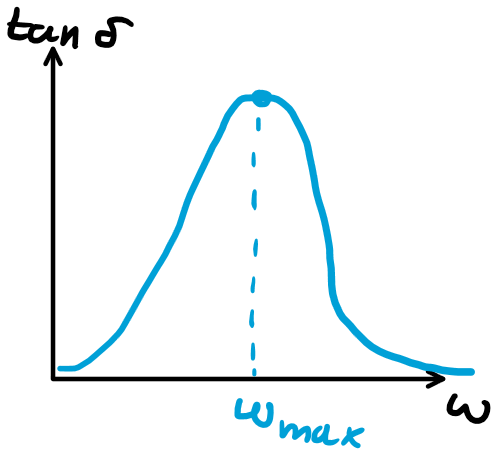
\includegraphics[width = 0.5\textwidth]{gfx/FattorePerdita}
\caption{Andamento del fattore di perdita per il modello \eng{Zener}}
\label{fig:FattorePerdite}
\end{figure}

Tra l'altro il picco si trova in corrispondenza di $\omega_{max}$ definito come:
\begin{equation}
\omega_{max} = \sqrt{\frac{1}{\tau_r\tau_c}}
\end{equation}

Sebbene il modello di \eng{Zenere} rappresenti bene i due comportamenti: nella realtà non è perfettamente rappresentativo di materiali viscoelastici.

\paragraph{Confronto coi dati sperimentali}
Il modello non riesce a raggiungere i valori ottenuti da una prova sperimentale. Funzionano qualitativamente ma non numericamente.
Alla figura \ref{fig:ConfSperimentale} viene rappresentato il confronto tra i dati ottenuti dalla prova sperimentale e il modello di \eng{Zener}.

\begin{figure}
\centering
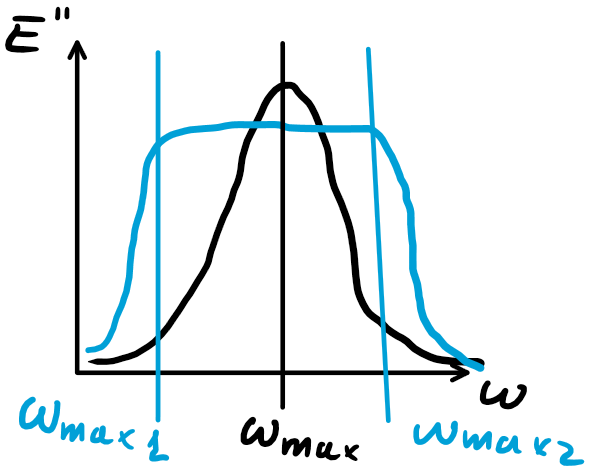
\includegraphics[width = 0.5\textwidth]{gfx/ConfSperimentale}
\caption{Confronto tra i dati sperimentali (in blu), e il modello di \eng{Zener}(in nero)}
\label{fig:ConfSperimentale}
\end{figure}

\begin{quote}
\emph{Si può correggere?}
\end{quote}
Considerando che il materiale rappresenta un comportamento dissipativo per un certo range di frequenze allora: mettendo in serie più modelli con tempo di rilassamento diverso:

\begin{equation}
\begin{split}
E(t) &= E_{\infty} + (E_0-E_{\infty})e^{-\frac{t}{\tau_r}}\\
E(t) &= E_{\infty} + K_1e^{-\frac{t}{\tau_{r_1}}} + K_2e^{-\frac{t}{\tau_{r_2}}} + \dots + K_Ne^{-\frac{t}{\tau_{r_N}}}\\
&= E_{\infty} + \sum_{i=1}^N{K_ie^{-\frac{t}{\tau_{r_i}}}}
\end{split}
\end{equation}

Il modello di \eng{Zener} corretto presenta uno spettro discreto di tempi di rilassamento. Uno per ogni elemento aggiuntivo inserito.\\
\graffito{\textbf{N.B.} Per ogni elemento aggiunto si introducono nuove variabili che devono essere ottenute sperimentalmente.}

In letteratura sono state sviluppati dei modelli adatti solo per rappresentare numericamente il comportamento dei dati sperimentali.
\textbf{Non fanno riferimento ad alcun sistema fisico}.

\begin{figure}
\centering
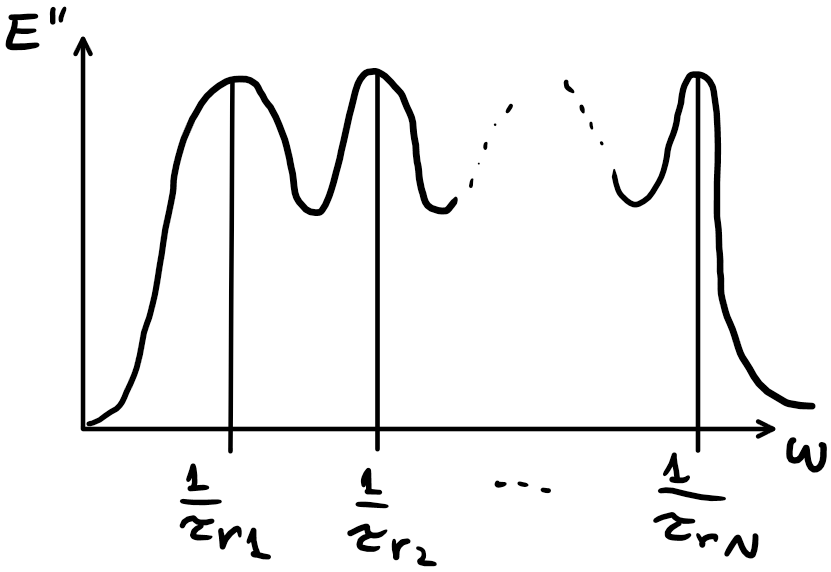
\includegraphics[width = 0.5\textwidth]{gfx/ZenerMod}
\caption{Modello di \eng{Zener} modificato per adattarsi ai dati sperimentali}
\label{fig:ZenerMod}
\end{figure}

\paragraph{Altri modelli}
\begin{description}
\item[$E(t) = E_{\infty} + \frac{E_0 - E_{\infty}}{\left(+\frac{t}{\tau_r}\right)^2}$] usata perché allarga il punto di massimo.
\item[$E(t) = E_{\infty} + \left(E_0 - E_{\infty}\right)e^{-\left(\frac{t}{\tau_r}\right)^\alpha}$] Sempre un modello a quattro parametri.
\item[$E(t) = E_{\infty}\left(1+\int_{t_1}^{t_2}{\frac{c}{\tau}e^{-\frac{t}{\tau}}\,d\tau}\right)$] Spettro continuo di tempi di rilassamento.
\end{description}

%************************************************
\chapter{Sovrapposizione tempo-temperatura}\label{chp:SovrapposizioneTT}
%************************************************
Ogni materiale viscoelastico viene caratterizzato dall'aumento della temperatura non si ha un decadimento della curva di rilassamento, bensì si sposta verso sinistra.

\begin{figure}
\centering
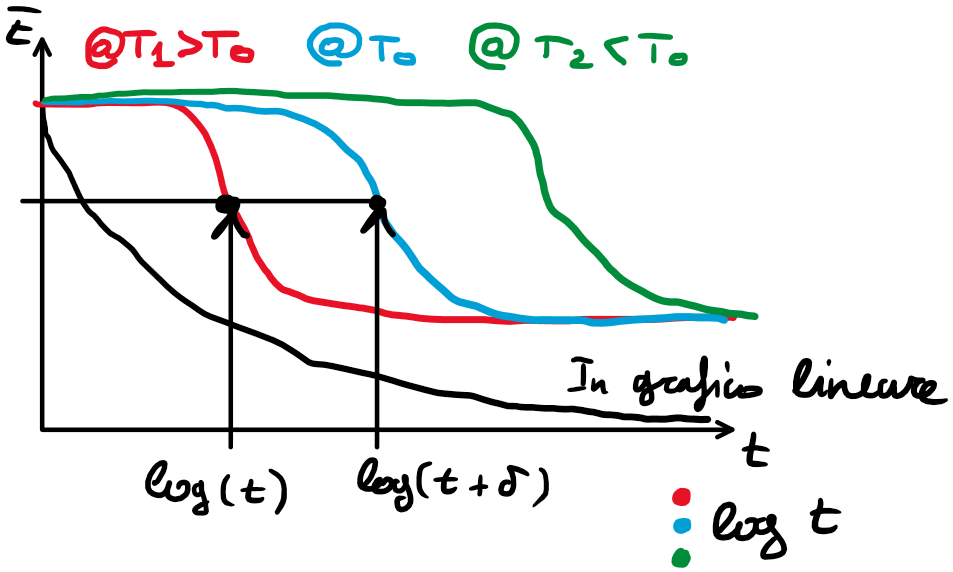
\includegraphics[width = \textwidth]{gfx/SovrapposizioneTT}
\caption{Comportamento di un materiale viscoelastico in diverse condizioni di temperatura, $T_0$ può essere la temperatura ambientale}
\label{fig:SovrapposizioneTT}
\end{figure}

Ciò è dovuto alla temperatura che aumentando dà più energia alle molecole, che saranno libere di svincolarsi tra loro più facilmente.
Da cui possiamo analiticamente descrivere:
\begin{equation}
E(\log(t),T_1) = E(\log(t+\delta), T_0)
\end{equation}
Imponiamo che $\delta = \log(\phi(T_1,T_0))$.
Allora definiamo la \textbf{funzione di \eng{shift}}:
\begin{equation}
a = a(T_1,T_0) = \frac{1}{\phi}
\end{equation}
Perciò:
\begin{equation}
\begin{split}
E(\log(t),T_1) &= E(\log(\phi(t)),T_0)\\
E(\log(t),T_1) &= E(\log(\frac{t}{a}),T_0)\\
E(t,T_1) &= E(\frac{t}{a},T_0)
\end{split}
\end{equation}
Questa è l'equazione di \textbf{sovrapposizione tempo-temperatura}.

Quello che succede ad una temperatura più alta è esattamente ciò che succede ad una temperatura più bassa in maggior tempo.

\paragraph{Funzione di \eng{shift}}
La funzione di \eng{shift} è una funzione decrescente nella temperatura.
Viene rappresentata in figura \ref{fig:Shift}.
\begin{figure}
\centering
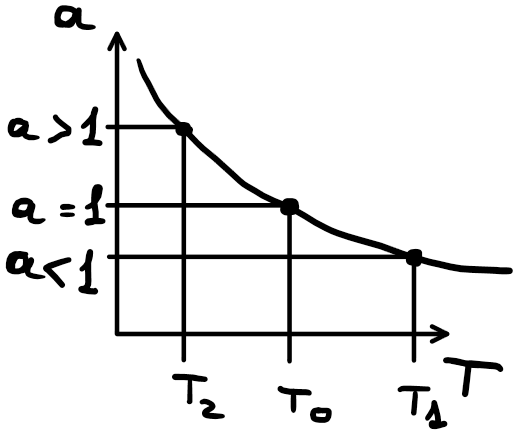
\includegraphics[width = 0.5\textwidth]{gfx/Shift}
\caption{Funzione di \eng{shift}}
\label{fig:Shift}
\end{figure}

\begin{quote}
\emph{$T_0$ viene presa come la temperatura ambiente?}
\end{quote}
Non per forza, ad esempio spesso viene usata come riferimento la temperatura di transizione vetrosa: $T_0=T_g$.
Dunque, si può pensare di realizzare delle prove proprio alla temperatura $T_g$.
Allora:
\begin{equation}
a(T,T_g) \Rightarrow \log(a) = \frac{-C_1(T-T_g)}{C_2 + T -T_g}
\end{equation}
Dove, $C_1$, $C_2$ sono costanti universali, comuni per tutti i polimeri.
\begin{equation}
C_1 = 17.4 \qquad C_2 = 51.6\unit{\kelvin}
\end{equation}

\section{Teoria di \eng{Williams-Landel-Ferry} (WLF)}
Questa teoria si propone di determinare una funzione di \eng{shift} indipendentemente dal polimero che si sta analizzando.

La teoria di \ac{WLF} funziona abbastanza bene per i materiali polimerici amorfi. 
Meno bene per i materiali semi-cristallini allora bisogna determinare sperimentalmente le due costanti $C_1$, $C_2$.

\begin{quote}
\emph{Si può sfruttare la teoria \ac{WLF} per effettuare delle prove accelerate?}
\end{quote}
Si sfrutta la teoria per ottenere i pezzi mancanti per completare la curva alla temperatura di riferimento.
Si effettuano diverse prove a temperatura più o meno alte. Poi si traslano i pezzi di curva in scala logaritmica per completare la \textbf{master curve}.
Un esempio è quello della figura \ref{fig:WLF}.

Variando la temperatura si può vedere ciò che succederebbe al materiale a tempo molto più lungo.
Si possono effettuare delle prove sinusoidali dove si mantene costante la frequenza, ad esempio $1\unit{\hertz}$.
Invece di modificare la frequenza, si modifica la temperatura.

\begin{figure}
\centering
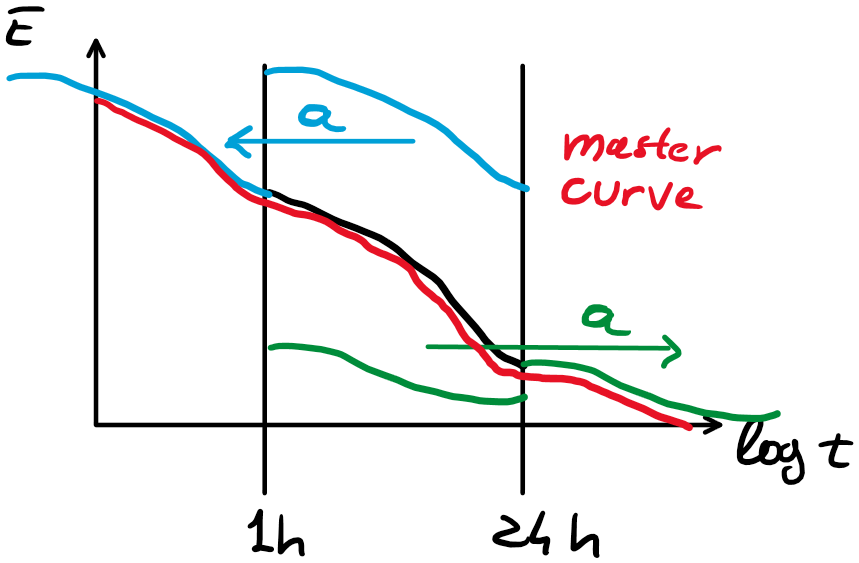
\includegraphics[width = 0.5\textwidth]{gfx/WLF}
\caption{Costruzione della \eng{master curve} grazie alla teoria \ac{WLF}}
\label{fig:WLF}
\end{figure}

\section{\eng{Dynamic-Mechanical Termic Analisys}}
La \ac{DMTA} è un'analisi molto accurata per misurare la temperatura di transizione vetrosa. Vedi figura \ref{fig:DMTA}.
In generale, durante la transizione vetrosa si ha un forte comportamento dissipativo da parte del materiale.
Dunque, si guarda al punto di massimo assoluto nella componente dissipativa $E"$ a cui corrisponderà la temperatura di transizione vetrosa $T_g$.

Nei materiali polimerici si fanno queste prove a materiale fluido.
Per cui, non si eseguono delle vere e proprie prove di trazione.
Piuttosto si considera un'equivalenza con degli sforzi torsionali e si impone una storia di sforzi in senso torsionale.

La \ac{DMTA} si sfrutta in particolare per i polimeri semi-cristallini.
Per gli amorfi si può stimare con la \ac{WLF} vista in precedenza.

\begin{figure}
\centering
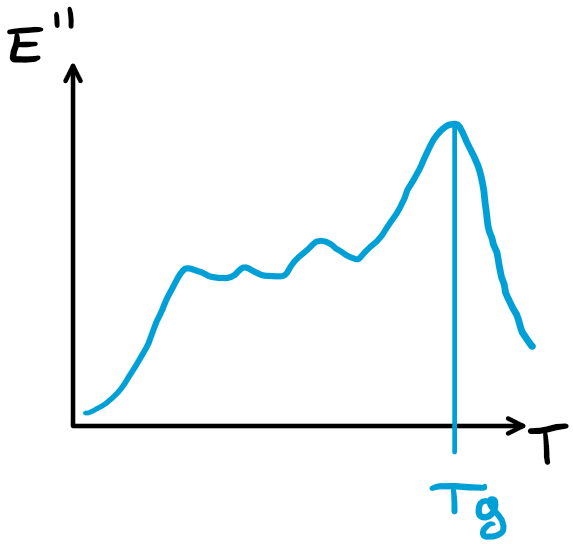
\includegraphics[width = 0.5\textwidth]{gfx/DMTA}
\caption{Grafico uscente dalla \ac{DMTA}}
\label{fig:DMTA}
\end{figure}